%!TEX root = ../dissertation.tex
\chapter{Introduction}
\label{introduction}

In the last years the scientific community made significant progress
in the development of models for solving computer vision and natural
language processing tasks. The reasons behind those outstanding
advancements are manifold. In first place, the constant increase of
computational resources allows to exploit complex models which can
capture intricate behaviour. Secondly, the availability of new data
speed-up the learning process in terms of how we can benefit from
available information. However, the joint understanding of both
modalities is still an hard task, specially if we constraint the
problem within a deliberately simple and human-like environment.

Both visual and language modalities are required for solving
interesting, challenging and community worthwhile problems such us
visual question answering, image retrieval, robotic navigation and
visual grounding \todo{CITE PAPERS}. Among these, visual grounding
task is a foundamental building block and can be used to postulate
other tasks as a variation of the latter. A first abstract definition
for visual grounding could be:

\begin{quote}
    \textit{The task of locating the content of the image referenced
    by a given sentence.}
\end{quote}

With the availability of large datasets \todo{CITE DATASET PAPERS},
many different solution for the visual grounding task has been
proposed in literature, but most of them relies on expensive
annotations. We argue that this technique cannot scale and is becoming
a critical bottlenck: it is hard and expensive to collect grounding
information while very simple to collect images with their
descriptions. Also, the way humans learn phrase localization is by
assembling prior kwnowledge instead of memorize a mapping between
textual and image examples.

This encourages us to investigate the visual grounding task under the
weakly supervised setting. In weakly supervised scenario, the
available ground truth is a shallow information which links a
description with its own image and vice-versa. On the countraty, the
fully supervised setting provide also the information between noun
phrases and objects in image, while in unsupervised settings no ground
truth is available.

In this work, we propose a model for exploiting semantic information
convoyed by class labels on bounding box. We assert that, given a
phrase, the image should contain an object detected by an object
detector whose bounding box class label is similar to the head of
given phrase. \todo{rivedere la forma}

\section{Visual Grounding}

Visual grounding is the general task of locating the components of a strucutred description in an image. 

Take for example the image in Fig.~\ref{fig:dog-playing-with-ball} and
the phrase ``A collie plays with a white ball in a field of green
grass''. We can think to many solutions for the visual grounding
problem given that input. A first approach would be to grossly
localize the subject of the phrase in the image, thus, pratically
speaking, to draw a coarse box around the dog playing with the ball
(red box). Another solution instead would be to localize the ball, the
dog and the ground distinctly, identifying precise regions of the
image and draw precise boxes among interesed objects. Both two
solutions are legal and belong to the visual grounding field. The
former is known as referring expression grounding (REG) while the
latter as phrase grounding (PG). The main difference between the two
is the grain used to solve the problem, and this has significant
impacts on how we can approach the problem and the relevance for other
tasks.
\todo{add "see section XX" for more details.}

\begin{figure}
    \centering
    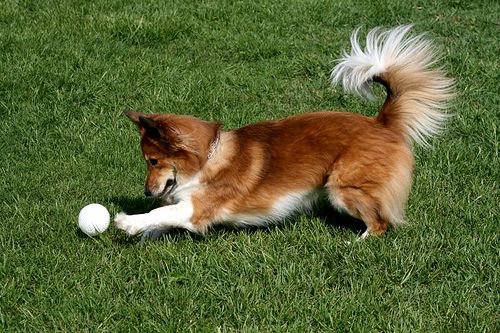
\includegraphics[width=0.7\textwidth]{resources/dog-playing-with-ball.jpg}
    \caption[Short figure name.]{This is a figure that floats inline and here is its caption. \todo{complete description and add two images, one for reg and the other for phrase grounding}
    \label{fig:dog-playing-with-ball}}
\end{figure}

\newthought{Referring Expression Grounding} is the task of locating
the subject referred by an expression an given image. 

More formally,
given in input an image $\bm{I}$ and a sentence $\mathrm{S}$, REG
consists in learning a function $\delta$ from the set $\calS$ of
sentences to a set of bounding boxes $B$ defined on $\bm{I}$, i.e.,
$\delta: \calI \times \calS \rightarrow 2^{\calS \times \calB}$, where
$\calI$ is the domain of images, $\calS$ is the domain of sentences,
$\calB$ is the domain of bounding boxes which can be defined on
$\calI$, and $2^{\calS \times \calB}$ is the power set of the
cartesian product between $\calS$ and $\calB$. In our example, ``the
dog'' is the referred expression and the red bounding box is the
correct solution.

\newthought{Phrase Grounding}, instead, is the task that studies the
mapping from noun phrases to regions of an image. In order to solve
this task, first, it is necessary to recognize all the objects in the
image and the components in the text, while after, the model needs to
find the correct alignment among the nouns and the objects.

More formally, given in input an image $\bm{I}$ and a sentence
$\mathrm{S}$, phrase grounding consists in learning a mapping $\gamma$
from the set $\calQ$ of noun phrases to a set of bounding box $\calB$
defined on $\bm{I}$, i.e., $\gamma : \calI \times \calS \rightarrow
2^{\calQ \times \calB}$. 

So, given an image $\bm{I}$ containing e objects identified via the
set of bounding boxes $B_\calI = \{ b_i \}^e_{i=1}$, where $b_i \in
\Rset^4$ is the vector of coordinates identifying a bounding box in
$\bm{I}$, and a sentence $\mathrm{S}$ containing $m$ noun phrases
gathered in the set $\calQ_S = \{ q_j \}^m_{j=1}$, where $q_j \in
\Nset^2$ is a vector containing as coordinates the initial and final
character positions in the sentence $\mathrm{S}$, $\gamma(\bm{I},
\mathrm{S})$ returns a set of couples $\{ (\bm{q}, \bm{b}) \mid \bm{q}
\in \calQ_{\mathrm{S}}, \bm{b} \in B_{\bm{I}} \}$ where each couple
$(\bm{q}, \bm{b})$ associates the noun phrase $\bm{q}$ to the bounding
box $\bm{b}$. Please, notice that the same noun phrase can be
associated to several different bounding boxes, as well as the same
bounding box can be associated to many different noun phrases.
Following the current literature, in this paper we assume that each
noun phrase is associated to one and only one bounding box. Bounding
boxes, however, can identify more objects, e.g. several persons in the
case the noun phrase is ``people''.

In the rest of our work we will focus on phrase grounding, as it is considered the foundamental building block for many high-level computer vision tasks such as image retrieval, QA, video QA, etc. \todo{cite kwnowledge aided consistency}.

\cite{conser2019revisiting} \todo{FIX CITE}

\section{One Stage vs Two Stage}

TODO

\section{Fully/Weakly/Self/Un-Supervised Settings}

TODO
